To evaluate the effectiveness of \TRANPCNN, we conduct experiments on open source software projects and compare it with several state-of-the-art bug localization methods.

\subsection{Research Questions}
%\dl{Ferdian, please add details on why the RQs are interesting and the purpose of the RQs}

Our experiments are designed to address the following research questions:

\vspace{0.2cm}\noindent\textit{\textbf{RQ1}: Is there a need for a specialized technique for cross-project bug localization?}

If a model learned from one project can be used for other projects, then there is no need for a specialized technique for cross-project bug localization. Thus, before we consider other research questions, we validate the need for our proposed approach by empirically evaluating the effectiveness of a model learned from one project to localize bugs in other projects.

\vspace{0.2cm}\noindent\textit{\textbf{RQ2}: Do the project-specific prediction layer improve the bug localization performance?}

%\dl{Xuan, please help to motivate this research question. I can't motivate it since I believe the details of the approach is going to change.}

In Section 3, we propose to employ project-specific prediction layer that apply two fully-connected networks for prediction from source and target projects separately, which is the key part of \TRANPCNN. In this research question, we evaluate whether the layer improves the bug localization performance by comparing the results with NP-CNN.

\vspace{0.2cm}\noindent\textit{\textbf{RQ3}: Can \TRANPCNN outperform other bug localization methods?}

A number of bug localization methods have been proposed in the literature. In this research question, we evaluate whether and to what extent can our proposed approach \TRANPCNN outperforms the state-of-the-art methods designed for bug localization and those that can be adapted for bug localization. 

\subsection{Datasets}
We consider three datasets containing a total of 5,591 reports from JIRA issue tracking systems of HTTPClient (H)\footnote{\url{http://hc.apache.org/httpcomponents-client-ga/index.html}}, Jackrabbit (J)\footnote{\url{https://jackrabbit.apache.org/jcr/index.html}}, and Lucene-Java (L)\footnote{\url{ http://lucene.apache.org/}}. HTTPClient is a library for implementing the client side of HTTP standard, while Jackrabbit is a content repository, and Lucene is a text search engine. We only consider projects with JIRA issue tracking systems since links between bug reports and their bug fixing commits stored in them are typically more reliable than those stored in Bugzilla issue tracking systems -- c.f.,~\cite{BissyandeTWLJR13}. The details of the reports considered in this study are shown in Table~\ref{tab:reports} and they have been used before by Kochhar et al.~\cite{KochharTL14}. 

\begin{table}
\caption{Bug Report Dataset}\label{tab:reports}
\begin{tabular}{|l|l|l}
\hline
{\bf Project} & {\bf \# Reports} \\
\hline HTTPClient & 746\\
\hline Jackrabbit & 2,402\\
\hline Lucene-Java & 2,443\\
\hline
\end{tabular}
\end{table}

\dl{Xuan, I thought we are also using your previous datasets? If we only use Pavneet's dataset, do we use all of them or only some of them that are not biased? Pavneet showed that some of the dataset is biased ... reviewers may be concerned with this bias ... Bias 2 mentioned in this paper (\url{http://ink.library.smu.edu.sg/cgi/viewcontent.cgi?article=3425&context=sis_research}) is particularly important.}

\xh{Currently we only use Paveneet's datasets (H,J and L), and yes we have considered the bias, and we only use the unbiased data sets. The ``fully localized'' bug reports are filtered. Our previous data sets are bias, so we are not sure if we use here is suitable.  If necessary, we can conduct several comparison experiments ono more data sets. }

%\dl{Ferdian, please add details datasets. Please see the following papers for details of the datasets:~\cite{huo2016learning,KochharTL14}.}



\subsection{Evaluation Metrics}
%The evaluation metrics are presented here. %\dl{Ferdian, please add details on evaluation metrics.}

Following prior bug localization studies~\cite{SahaLKP13,SahaLKP14,zhou2012should,huo2016learning}, we consider three evaluation metrics: Top-N, Mean Average Precision (MAP), and Mean Reciprocal Rank. Their brief definitions considering the context of bug localization are given below:

\vspace{0.2cm}\noindent{\bf Top-N.} Top-N reports the proportion of bug reports for which one of the buggy files appear in the top-N position in the ranked list returned by a bug localization tool. Following prior studies~\cite{SahaLKP13,SahaLKP14,zhou2012should,huo2016learning}, we consider three values of N, i.e., 1, 5, and 10. This is further motivated by the findings of Kochhar et al.~\cite{KochharXLL16} which highlight that more than 95\% of practitioners would not check beyond the top-10 results of a bug localization tool.

\vspace{0.2cm}\noindent{\bf Mean Average Precision (MAP).} For each ranked list produced by a bug localization technique for a bug report, we can compute its average precision (AP) as follows:

\begin{equation}
\sum_{i} \frac{P(i)\times isBuggy(i)}{\# buggy files}
\end{equation}

In the above equation, $\mathit{P(i)}$ is the precision at position $i$ (i.e., proportion of files at position 1 to $i$ that are buggy), while $\mathit{isBuggy(i)}$ is 1 if the file at position $i$ is buggy and 0 otherwise. The denominator of the equation is the number of buggy files in the entire ranked list. MAP is the mean of APs considering all bug reports.

\vspace{0.2cm}\noindent{\bf Mean Reciprocal Rank (MRR).} For each ranked list produced by a bug localization technique for a bug report, we can compute the position of the first buggy file. The reciprocal of such position is referred to as the reciprocal rank (RR). MRR is the mean of RRs considering all bug reports.



\subsection{Baselines}

We compare our proposed model \TRANPCNN with following baseline methods:
\begin{itemize}
  \item VSM (Vector Space Model)~\cite{rao2011retrieval}: a baseline method that firstly uses Vector Space Model to represent the text bug reports and source code, then employs Logistic Regression to predict the related buggy source code.
  \item Burak (Burak Filter)~\cite{peters2013better}: a state-of-the-art method for cross-project and cross-company defect prediction problem, which filters training sets using Burak filter that employs k-nearest neighbour to selects instances in the source project similar to the test project.
  \item TCA+ (Transfer Component Analysis)~\cite{NamPK13}: a state-of-the-art transfer learning method in software engineering, which firstly normalizes the data and employs TCA to map source and target project into a same feature space and then apply Logistic Regression for bug localization (same settings suggested in their paper). 
  \item TCA+$^{(P)}$ (Transfer Component Analysis with multi-layer Perceptron): a state-of-the-art transfer learning method in software engineering, which firstly normalizes the data and employs TCA to map source and target project into a same feature space and then apply MLPs for bug localization (same settings with fully-connected layers in \TRANPCNN).
   \item TCA+$^{(D)}$ (Transfer Component Analysis with Deep features): a state-of-the-art transfer learning method in software engineering, which firstly normalizes the data and employs TCA to map source and target project into a same feature space and then apply Logistic Regression for bug localization (using deep features extracted from CNN instead of VSM features).
  \item NP-CNN (Natural and Programming language Convolutional Neural Network)~\cite{huo2016learning}: a state-of-the-art deep model for bug localization, which uses source project data for training a deep convolutional neural network and localizes the buggy source code for target project data.
\end{itemize}
%\ft{Settings would probably better be grouped in experimental settings section. There is no citation for TCA. }

\subsection{Experimental Settings}
First, the parameter settings of baseline methods (VSM, burak, TCA+, TCA+$^{(P)}$, TCA+$^{(D)}$), we use the same parameters settings suggested in their work~\cite{rao2011retrieval}\cite{NamPK13}. The parameters are set the same in~\cite{huo2016learning}. 

For the \TRANPCNN model, we employ the most commonly used ReLU $\sigma(x)=\max(0,x)$ as active function and the filter windows size $d$ is set as 3, 4, 5, with 100 feature maps each in Within-Project feature extraction layers. The number of neurons in fully-connect network in  set the same number of CNN. In addition, the drop-out method is also applied which is used to prevent co-adaption of hidden units by randomly dropping out values in fully-connected layers, and the drop-out probability $p$ is set 0.25 in our experiments.

For data partition, we use data from source projects and 20\% target projects as training sets, and locates the 80\% buggy code in target projects. This process repeats for 5 times to reduce the influence of randomness, and we report the average results for comparison. 

\section{Experimental Results}

\subsection{Experimental Results for Research Questions}

\begin{table}[htbp]
  \centering
  \caption{Performance Comparisons between within-project and cross-project bug localization.}
  \resizebox{!}{0.5\columnwidth}{
    \begin{tabular}{c|l|c|c|c|c|c}
    \toprule
    Tasks & \textit{Methods} & \multicolumn{1}{l}{\textit{Top 1}} & \multicolumn{1}{l}{\textit{Top 5}} & \multicolumn{1}{l}{\textit{Top 10}} & \multicolumn{1}{l}{\textit{MAP}} & \multicolumn{1}{l}{\textit{MRR}} \\
    \midrule
    \multirow{3}[0]{*}{\textbf{J}$\rightarrow$\textbf{H}} & NPCNN & 0.317  & 0.362  & 0.508  & 0.276  & 0.352  \\
          & NPCNN$^{partial}$ & 0.204  & 0.258  & 0.313  & 0.202  & 0.292  \\
          & NPCNN$^{full}$ & \textbf{0.533}  & \textbf{0.617}  & \textbf{0.650}  & \textbf{0.472}  & \textbf{0.580}  \\
          \midrule
    \multirow{3}[0]{*}{\textbf{L}$\rightarrow$\textbf{H}} & NPCNN & 0.142  & 0.192  & 0.345  & 0.161  & 0.218  \\
          & NPCNN$^{partial}$ & 0.204  & 0.258  & 0.313  & 0.202  & 0.292  \\
          & NPCNN$^{full}$ & \textbf{0.533}  & \textbf{0.617}  & \textbf{0.650}  & \textbf{0.472}  & \textbf{0.580}  \\
          \midrule
    \multirow{3}[0]{*}{\textbf{H}$\rightarrow$\textbf{J}} & NPCNN & 0.167  & 0.287  & 0.349  & 0.247  & 0.277  \\
          & NPCNN$^{partial}$ & 0.035  & 0.211  & 0.302  & 0.155  & 0.189  \\
          & NPCNN$^{full}$ & \textbf{0.508}  & \textbf{0.587}  & \textbf{0.679}  & \textbf{0.462}  & \textbf{0.557}  \\
          \midrule
    \multirow{3}[0]{*}{\textbf{L}$\rightarrow$\textbf{J}} & NPCNN & 0.152  & 0.182  & 0.318  & 0.176  & 0.221  \\
          & NPCNN$^{partial}$ & 0.035  & 0.211  & 0.302  & 0.155  & 0.189  \\
          & NPCNN$^{full}$ & \textbf{0.508}  & \textbf{0.587}  & \textbf{0.679}  & \textbf{0.462}  & \textbf{0.557}  \\
          \midrule
    \multirow{3}[0]{*}{\textbf{H}$\rightarrow$\textbf{L}} & NPCNN & 0.173  & 0.246  & 0.390  & 0.196  & 0.329  \\
          & NPCNN$^{partial}$ & 0.097  & 0.219  & 0.335  & 0.095  & 0.109  \\
          & NPCNN$^{full}$ & \textbf{0.289}  & \textbf{0.484}  & 0.611  & \textbf{0.287}  & \textbf{0.387}  \\
          \midrule
    \multirow{3}[0]{*}{\textbf{J}$\rightarrow$\textbf{L}} & NPCNN & 0.110  & 0.255  & 0.323  & 0.141  & 0.176  \\
          & NPCNN$^{partial}$ & 0.097  & 0.219  & 0.335  & 0.095  & 0.109  \\
          & NPCNN$^{full}$ & \textbf{0.289}  & \textbf{0.484}  & \textbf{0.611}  & \textbf{0.287}  & \textbf{0.387}  \\
          \bottomrule
    \end{tabular}%
    }

  \label{tab:results1}%
\end{table}%


\begin{figure}[hbt]
\centering
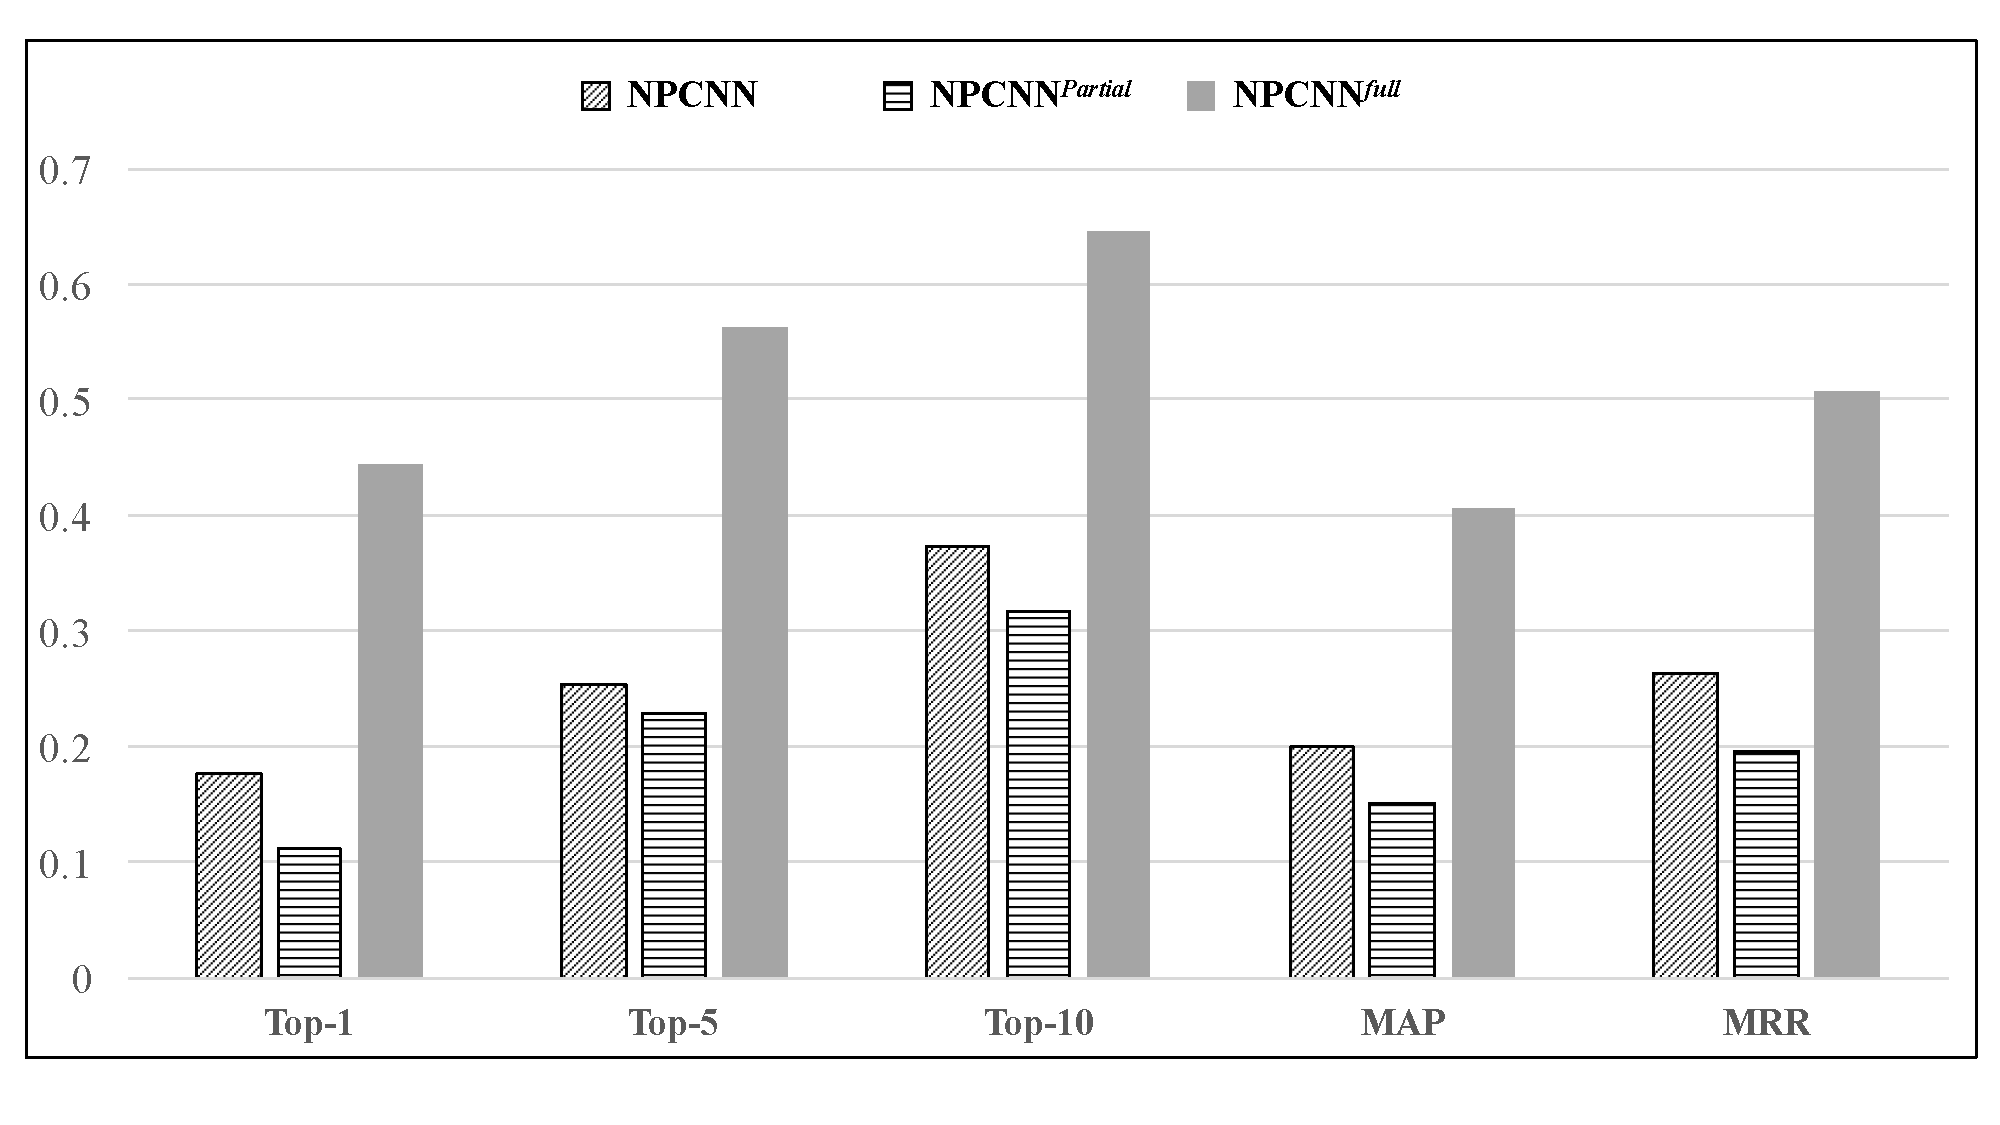
\includegraphics[width = 0.9\columnwidth]{pic/results1_avg.pdf}
\caption{Performance comparisons between within-project and cross-project bug localization.}
\label{fig:results1}
\end{figure}


\textbf{RQ1}: \textit{Is there a need for cross-project bug localization?}

To answer this research question, we compare the results of using NP-CNN for bug localization in different settings.

\begin{itemize}
  \item NPCNN: Employ NPCNN directly for cross-project bug localization, which means directly training the model on the data from source projects and locating the bugs in the target project.
  \item NPCNN$^{partial}$: Employ NPCNN using partial data of target projects, which means training based on a few data (20\%) in the target projects, and localizes target buggy files without using data from source project.
  \item NPCNN$^{full}$: Employ NPCNN using full data of target projects. In this setting, we conduct 5-folds cross-validation for comparison.
\end{itemize}

The results are detailed in Table.~\ref{tab:results1} and Figuire.~\ref{fig:results1}. There are six tasks in the table, in which $\textbf{H}$ represents project \textit{HTTPClient}, $\textbf{J}$ represents project \textit{Jackrabbit} and $\textbf{L}$ represents \textit{Lucene-Java}. Meanwhile, the task $\textbf{H} \rightarrow \textbf{J}$ represents using \textit{HTTPClient} as source project and predicts the location of buggy files in target project \textit{Jackrabbit}. The results show that the performance of bug localization using full data of target projects is the best, which has a large gap against the performance using partial data. For cross-project bug localization, the performance of NPCNN that directly uses source projects is better than NPCNN$^{partial}$, showing that cross-project data is beneficial to improve the bug localization performance, but directly using within-project bug localization technique will not as well as NPCNN$^{full}$. The results suggest that there is a need for cross-project bug localization, and directly using within-project bug localization method does not show good performance.

\textbf{RQ2}: \textit{Do the project-specific correlation fitting layers improve the bug localization performance?}

To answer this research question, we compare the results of \TRANPCNN with the original NPCNN. The difference of the structure between \TRANPCNN and NPCNN is that \TRANPCNN employs two fully-connected networks to combine deep features from source projects and target projects in the project-specific correlation fitting layers, respectively, which will counter the influences that cross-project data may have different distribution leading to a bias performance. The results are detailed in Tab.~\ref{tab:results2}.

%\ft{It would be good if we can explain why such structure can counter bias. Perhaps we should explain this first in approach (theory) and then highlight it again accompanied with experimental result (empirical).}

\begin{table}[htbp]
  \centering
  \caption{Performance comparisons with previous deep models.}
  \resizebox{!}{0.35\columnwidth}{
    \begin{tabular}{c|l|c|c|c|c|c}
    \toprule
    Tasks & \textit{Methods} & \textit{Top 1} & \textit{Top 5} & \textit{Top 10} & \textit{MAP} & \textit{MRR} \\
    \midrule
    \multirow{2}[0]{*}{\textbf{J}$\rightarrow$\textbf{H}} & NPCNN & 0.317  & 0.362  & 0.508  & 0.276  & 0.352  \\
%          & SimpleTrans & 0.354 & 0.396 & 0.563 & 0.298 & 0.395 \\
          & \TRANPCNN & \textbf{0.500}   & \textbf{0.583} & \textbf{0.625} & \textbf{0.376} & \textbf{0.543} \\
          \midrule
    \multirow{2}[0]{*}{\textbf{L}$\rightarrow$\textbf{H}} & NPCNN & 0.142  & 0.192  & 0.345  & 0.161  & 0.218  \\
%          & SimpleTrans & 0.163 & 0.146 & 0.354 & 0.141 & 0.246 \\
          & \TRANPCNN & \textbf{0.275} & \textbf{0.35}  & \textbf{0.488} & \textbf{0.242} & \textbf{0.332} \\
          \midrule
    \multirow{2}[0]{*}{\textbf{H}$\rightarrow$\textbf{J}} & NPCNN & 0.167  & 0.287  & 0.349  & 0.247  & 0.277  \\
%          & SimpleTrans & 0.133 & 0.324 & 0.365 & 0.273 & 0.301 \\
          & \TRANPCNN & \textbf{0.396} & \textbf{0.443} & \textbf{0.514} & \textbf{0.371} & \textbf{0.434} \\
          \midrule
    \multirow{2}[0]{*}{\textbf{L}$\rightarrow$\textbf{J}} & NPCNN & 0.152  & 0.182  & 0.318  & 0.176  & 0.221  \\
%          & SimpleTrans & 0.144 & 0.204 & 0.382 & 0.247 & 0.249 \\
          & \TRANPCNN & \textbf{0.460}  & \textbf{0.462} & \textbf{0.488} & \textbf{0.404} & \textbf{0.478} \\
          \midrule
    \multirow{2}[0]{*}{\textbf{H}$\rightarrow$\textbf{L}} & NPCNN & 0.173  & 0.246  & 0.390  & 0.196  & 0.329  \\
%          & SimpleTrans & 0.197 & 0.323 & 0.426 & 0.152 & 0.313 \\
          & \TRANPCNN & \textbf{0.361} & \textbf{0.445} & \textbf{0.535} & \textbf{0.279} & \textbf{0.414} \\
          \midrule
    \multirow{2}[0]{*}{\textbf{J}$\rightarrow$\textbf{L}} & NPCNN & 0.110  & 0.255  & 0.323  & 0.141  & 0.176  \\
%          & SimpleTrans & 0.140  & 0.282 & 0.342 & 0.163 & 0.224 \\
          & \TRANPCNN & \textbf{0.301} & \textbf{0.410}  & \textbf{0.517} & \textbf{0.247} & \textbf{0.368} \\
          \bottomrule
    \end{tabular}%
    }
  \label{tab:results2}%
\end{table}%

\begin{figure}[hbt]
\centering
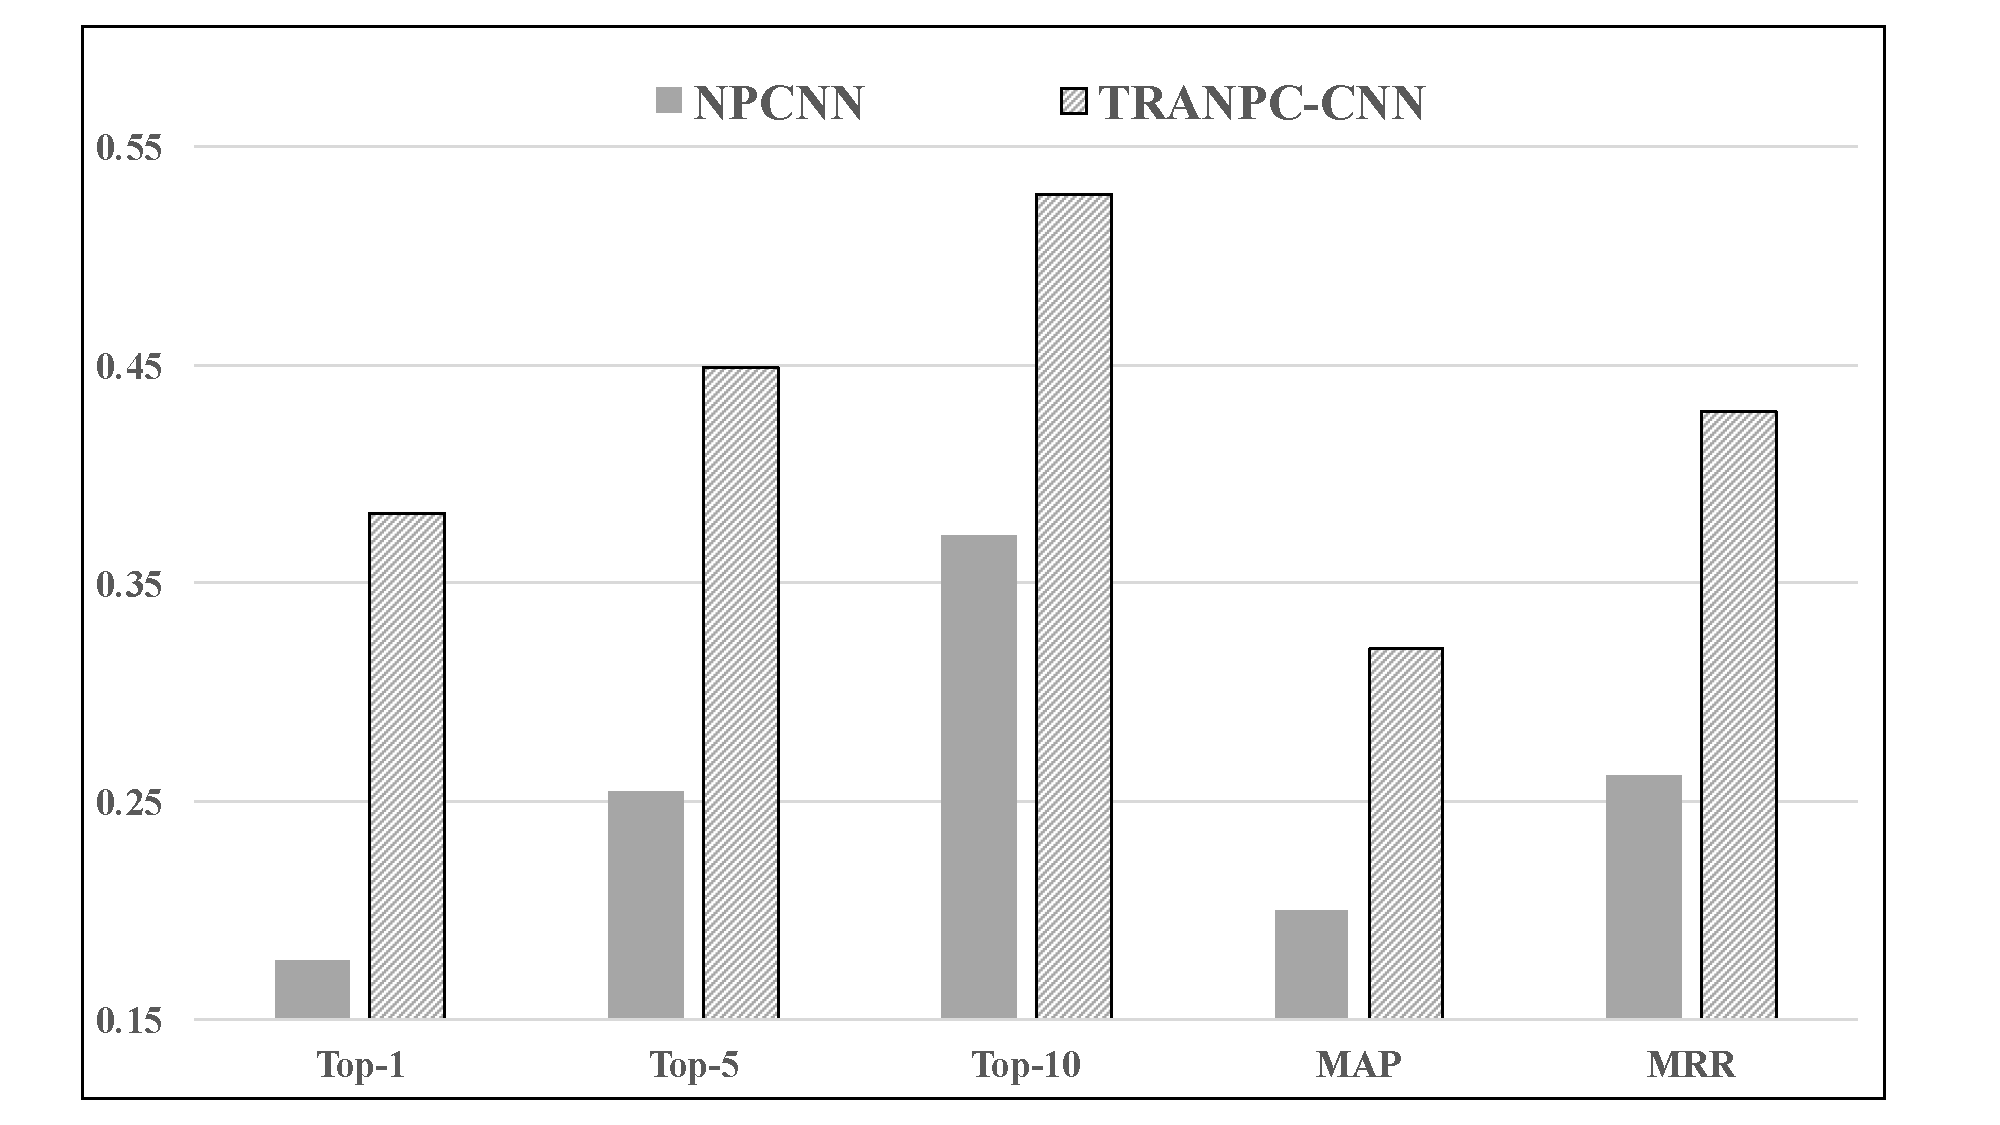
\includegraphics[width = 0.9\columnwidth]{pic/results2_avg.pdf}
\caption{Performance comparisons with deep models.}
\label{fig:results2}
\end{figure}

The results show that \TRANPCNN performs better than NP-CNN, which suggests that the project-specific correlation fitting layers  can improve the performance of cross-projects bug localization. It is because the project-specific correlation fitting layers employ two separate fully-connected network to learn the prediction function for each project separately to encounter the bias of data distribution and the results have provided the evidences.  

\textbf{RQ3}: \textit{Can \TRANPCNN outperform other bug localization methods?}

To answer this research question, we compare the results of \TRANPCNN with state-of-the-art methods: VSM, Burak, TCA+, TCA+$^(P)$. VSM is a baseline technique used in the within-project bug localization and we employ it on cross-project bug localization for comparison. Burak and TCA+ have been shown good performance on cross-project and cross-company defect prediction, and also we apply it on cross-project bug localization. The parameters of VSM and Burak Filter are set suggested in their work. For fair comparison with TCA+, we use same normalization strategy and the classifier in their original paper (Logistic Regression) and multi-layer perception (same as \TRANPCNN) are compared in our experiments. The results are detailed in Tab.~\ref{tab:results3}. 

%\ft{We should directly use abbreviations of baseline names since they have been introduced in Baselines section. Explanations about baselines are also redundant. }

According to the results, we have several findings: 1. Burak and TCA techniques perform better than the baseline VSM model, indicating that using transfer algorithms is able to improve the performance in cross-project bug localization; 2. \TRANPCNN outperforms TCA-P, which shows that the high-level features extracted from CNN are more semantic and informative, leading to a better representation and bug localization performance; 3. TCA-D uses deep features extracted from CNN and the performance is not as well as \TRANPCNN, which further proves that the cross-project feature fusion layers improve bug localization performance; 4. \TRANPCNN obtains the best average values in terms of all evaluation metrics. Comparing to the best baseline TCA+$^{(D)}$, \TRANPCNN improves the results by 24.6\% in terms of Top-1, by 22.6\% in terms of Top-5, by 20.9\% in terms of Top-10, by 21.9\% in terms of MAP and by 17.2\% in terms of MRR. According to Mann-Whitney U-test, we find \TRANPCNN significant better in terms of all metrics. The results suggest that \TRANPCNN outperforms other traditional bug localization methods and transfer techniques on software engineering.

%\ft{We can highlight the amount of improvement that \TRANPCNN achieves as compared to the best baseline.}

\begin{table}[htbp]
  \centering
  \caption{Performance comparisons with traditional bug localization models.}
  \resizebox{!}{0.9\columnwidth}{
    \begin{tabular}{c|l|c|c|c|c|c}
    \toprule
    Tasks & \textit{Methods} & \multicolumn{1}{c|}{\textit{Top 1}} & \multicolumn{1}{c|}{\textit{Top 5}} & \multicolumn{1}{c|}{\textit{Top 10}} & \multicolumn{1}{c|}{\textit{MAP}} & \multicolumn{1}{c}{\textit{MRR}} \\
    \midrule
    \multirow{6}[0]{*}{\textbf{J}$\rightarrow$\textbf{H}} & VSM   & 0.098  & 0.157  & 0.177  & 0.087  & 0.143  \\
          & Burak & 0.110  & 0.126  & 0.138  & 0.116  & 0.121  \\
          & TCA-R & 0.120  & 0.212  & 0.144  & 0.157  & 0.162  \\
          & TCA-P & 0.114  & 0.133  & 0.154  & 0.123  & 0.176  \\
          & TCA-D & 0.122  & 0.225  & 0.271  & 0.168  & 0.248  \\
          & \TRANPCNN & \textbf{0.500}  & \textbf{0.583}  & \textbf{0.625}  & \textbf{0.376}  & \textbf{0.543}  \\
          \midrule
    \multirow{6}[0]{*}{\textbf{L}$\rightarrow$\textbf{H}} & VSM   & 0.059  & 0.098  & 0.237  & 0.099  & 0.112  \\
          & Burak & 0.113  & 0.203  & 0.242  & 0.143  & 0.143  \\
          & TCA-R & 0.120  & 0.188  & 0.244  & 0.151  & 0.158  \\
          & TCA-P & 0.128  & 0.200  & 0.252  & 0.161  & 0.167  \\
          & TCA-D & 0.102  & 0.237  & 0.367  & 0.161  & 0.202  \\
          & \TRANPCNN & \textbf{0.275}  & \textbf{0.350}  & \textbf{0.488}  & \textbf{0.242}  & \textbf{ 0.332}  \\
          \midrule
    \multirow{6}[0]{*}{\textbf{H}$\rightarrow$\textbf{J}} & VSM   & 0.035  & 0.211  & 0.232  & 0.165  & 0.129  \\
          & Burak & 0.130  & 0.150  & 0.206  & 0.225  & 0.195  \\
          & TCA-R & 0.115  & 0.162  & 0.209  & 0.239  & 0.244  \\
          & TCA-P & 0.114  & 0.154  & 0.203  & 0.237  & 0.241  \\
          & TCA-D & 0.111  & 0.135  & 0.157  & 0.168  & 0.185  \\
          & \TRANPCNN & \textbf{0.396}  & \textbf{0.443}  & \textbf{0.514}  & \textbf{0.371}  & \textbf{0.434}  \\
          \midrule
    \multirow{6}[0]{*}{\textbf{L}$\rightarrow$\textbf{J}} & VSM   & 0.197  & 0.212  & 0.293  & 0.167  & 0.216  \\
          & Burak & 0.161  & 0.132  & 0.368  & 0.170  & 0.187  \\
          & TCA-R & 0.136  & 0.183  & 0.370  & 0.170  & 0.179  \\
          & TCA-P & 0.114  & 0.116  & 0.397  & 0.138  & 0.191  \\
          & TCA-D & 0.178  & 0.236  & 0.469  & 0.227  & 0.256  \\
          & \TRANPCNN & \textbf{0.460}  & \textbf{0.462}  & \textbf{0.488}  & \textbf{0.404}  & \textbf{0.478}  \\
          \midrule
    \multirow{6}[0]{*}{\textbf{H}$\rightarrow$\textbf{L}} & VSM   & 0.083  & 0.278  & 0.393  & 0.154  & 0.136  \\
          & Burak & 0.105  & 0.226  & 0.272  & 0.123  & 0.222  \\
          & TCA-R & 0.136  & 0.208  & 0.383  & 0.170  & 0.279  \\
          & TCA-P & 0.143  & 0.226  & 0.394  & 0.171  & 0.288  \\
          & TCA-D & 0.162  & 0.207  & 0.345  & 0.229  & 0.292  \\
          & \TRANPCNN & \textbf{0.361}  & \textbf{0.445}  & \textbf{0.535}  & \textbf{0.279}  & \textbf{0.414}  \\
          \midrule
    \multirow{6}[0]{*}{\textbf{J}$\rightarrow$\textbf{L}} & VSM   & 0.038  & 0.077  & 0.154  & 0.124  & 0.204  \\
          & Burak & 0.138  & 0.161  & 0.176  & 0.168  & 0.226  \\
          & TCA-R & 0.135  & 0.111  & 0.172  & 0.169  & 0.222  \\
          & TCA-P & 0.136  & 0.132  & 0.192  & 0.173  & 0.237  \\
          & TCA-D & 0.142  & 0.297  & 0.308  & 0.238  & 0.293  \\
          & \TRANPCNN & \textbf{0.301}  & \textbf{0.410}  & \textbf{0.517}  & \textbf{0.247}  & \textbf{0.368}  \\

          \bottomrule
    \end{tabular}%
    }
  \label{tab:results3}%
\end{table}%

\begin{figure}[hbt]
\centering
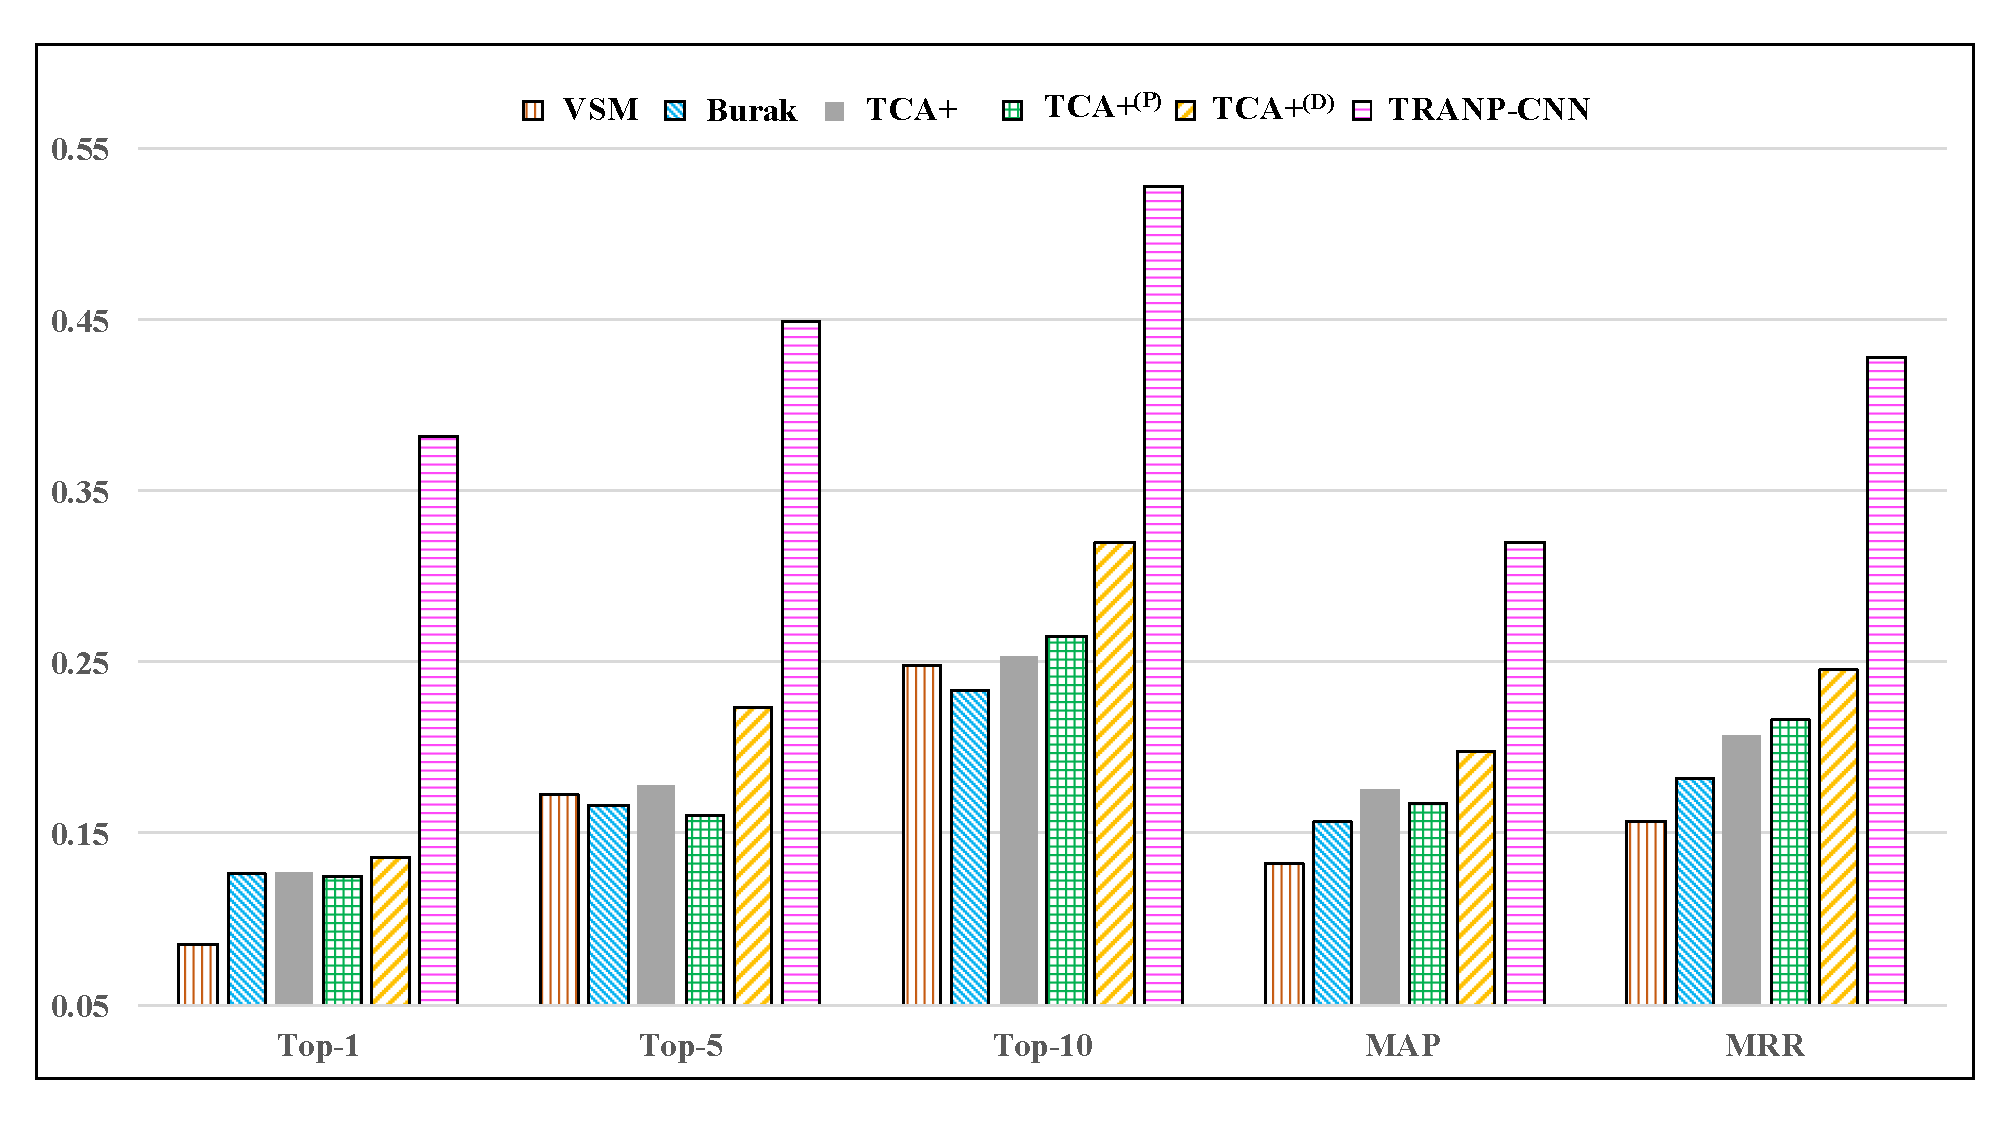
\includegraphics[width = 0.9\columnwidth]{pic/results3_avg.pdf}
\caption{Performance comparisons with traditional bug localization models.}
\label{fig:results3}
\end{figure}

